\documentclass[11pt]{article}

\usepackage[margin=1in]{geometry}
\usepackage{amsmath,amssymb,amsfonts,bm}
\usepackage{booktabs}
\usepackage{array}
\usepackage{longtable}
\usepackage{graphicx}
\usepackage{float}
\usepackage{caption}
\usepackage{subcaption}
\usepackage{enumitem}
\usepackage{hyperref}
\usepackage{xcolor}
\usepackage[nopatch=footnote]{microtype}
\usepackage{setspace}
\usepackage{mathtools}
\mathtoolsset{showonlyrefs=true}

\hypersetup{
  colorlinks=true,
  linkcolor=blue,
  citecolor=blue,
  urlcolor=blue
}

\setstretch{1.08}
\setlength{\parskip}{0.55em}
\setlength{\parindent}{0pt}

\newcommand{\safeincludegraphics}[2][]{%
\IfFileExists{#2}{\includegraphics[#1]{#2}}{%
\fbox{\begin{minipage}[c][0.28\textheight][c]{0.82\textwidth}
\centering
\textit{Figure file not available:} \texttt{\detokenize{#2}}\\[0.5em]
\small Replace this placeholder with the original figure file when compiling the full manuscript.
\end{minipage}}%
}%
}


\title{Hybrid Tree-Boosted Entropy Balancing with Hard Main-Effect Calibration for Nonlinear Interaction Balance}
\author{Joseph Kang\\\small Draft research manuscript}
\date{\today}

\begin{document}
\maketitle

\begin{abstract}
Entropy balancing reweights a sample to match prespecified target moments, but its performance depends on selecting appropriate balance functions. Main effects and raw pairwise products may not captur[...]
\end{abstract}

\textbf{Keywords:} entropy balancing; calibration weighting; boosting; decision trees; interaction balance; sample reweighting; survey calibration; missing data; nonlinear interactions; variable impor[...]

\newpage
\tableofcontents
\newpage

\section{Introduction}

Entropy balancing is a widely used method for constructing sample weights that match user-specified target moments. Given source-sample covariates and external target moments, the method finds weights[...] 

The strength of entropy balancing is also a limitation: the analyst must specify the balance functions. If the analyst supplies only main effects, the method balances only main effects. If the analyst[...]
\begin{equation*}
E\left[\frac{\exp\{a(|X_0X_1|-c)\}}{1+\exp\{a(|X_0X_1|-c)\}}\right],
\end{equation*}
which captures whether two variables are jointly extreme, regardless of the sign of the product.

This problem motivates a boosted extension of entropy balancing. The central idea is to retain the clear calibration structure of entropy balancing but allow the algorithm to search adaptively for int[...] 

This manuscript develops a hybrid version of tree-boosted entropy balancing. The proposed method has two layers:
\begin{enumerate}[leftmargin=2em]
\item \textbf{Hard calibration layer.} The analyst chooses a set of hard moments that must be preserved, such as main-effect target means. These moments are balanced exactly, up to numerical tolerance[...]
\item \textbf{Boosted interaction layer.} A sequence of shallow trees identifies additional regions where the current weighted sample differs from the target. The weights are updated within the tree l[...]
\end{enumerate}

The method is designed to answer a specific practical question: can we preserve classical calibration balance on a trusted set of moments while adaptively improving balance on nonlinear or interaction[...]


\subsection{Main contributions}

The manuscript makes five contributions.

First, it gives the boosted method an explicit optimization target. The method is formulated as a projected stagewise optimizer for a hard-constrained Kullback--Leibler dual objective over an additive[...] 

Second, it formulates tree-boosted entropy balancing using user-provided target moments. Earlier intuitive descriptions of tree-based reweighting often use target microdata or target weights. Here the[...] 

Third, it derives the multiplicative tree-leaf update from an entropy projection. For a fixed tree partition, the update
\begin{equation*}
\widetilde w_i \propto w_i \left(\frac{\mu_L}{p_L}\right)^\nu, \qquad x_i\in L,
\end{equation*}
where $p_L$ is the current source mass in leaf $L$, $\mu_L$ is the target mass, and $\nu$ is a learning rate, is not an arbitrary boosting rule. It is the entropy projection onto tree-leaf margins, wi[...] 

Fourth, it introduces a hard-projection step after each tree update. The hard projection solves another entropy projection problem, using the temporary tree-updated weights as base weights, and restor[...] 

Fifth, it presents a Kang--Schafer-style simulation study and a real-data-based ACS microdata analysis, including both main EB-offset and pairwise EB-offset hybrid boosted EB variants. The simulation [...]

\section{Classical entropy balancing}

\subsection{Basic calibration problem}

Let $i=1,\ldots,n$ index the source sample. Each unit has covariates $x_i\in\mathbb{R}^p$ and a base weight $q_i>0$, with
\begin{equation*}
\sum_{i=1}^n q_i=1.
\end{equation*}

Let $h(x_i)\in\mathbb{R}^K$ be a vector of user-specified balance functions. Examples include main effects, transformations, dummy variables, and interactions. Let
\begin{equation*}
\mu = E_T\{h(X)\}
\end{equation*}
be the user-specified target moment vector. The classical entropy balancing problem is
\begin{equation*}
\widehat w
=
\arg\min_{w_1,\ldots,w_n}
\sum_{i=1}^n w_i\log\left(\frac{w_i}{q_i}\right)
\end{equation*}
subject to
\begin{equation*}
\sum_{i=1}^n w_i h(x_i)=\mu,
\qquad
\sum_{i=1}^n w_i=1,
\qquad
w_i>0.
\end{equation*}

The objective is the Kullback-Leibler distance from the new weights to the base weights. Thus the method chooses the closest weights to $q_i$ among those satisfying the target moment constraints.

\subsection{Exponential-tilting form}

When the problem is feasible and regular, the solution has an exponential-tilting form:
\begin{equation*}
\widehat w_i(\lambda)
=
\frac{q_i\exp\{\lambda^\top h(x_i)\}}
{\sum_{\ell=1}^n q_\ell\exp\{\lambda^\top h(x_\ell)\}}.
\end{equation*}
The Lagrange multiplier $\lambda$ is chosen so that
\begin{equation*}
\sum_{i=1}^n \widehat w_i(\lambda)h(x_i)=\mu.
\end{equation*}

The corresponding dual objective is
\begin{equation*}
\phi(\lambda)
=
\log\left[\sum_{i=1}^n q_i\exp\{\lambda^\top h(x_i)\}\right]-\lambda^\top\mu.
\end{equation*}
Its gradient is
\begin{equation*}
\nabla\phi(\lambda)=\sum_{i=1}^n \widehat w_i(\lambda)h(x_i)-\mu.
\end{equation*}
Thus the first-order condition is exactly the moment-balance condition.

\subsection{What classical entropy balancing can and cannot balance}

Classical entropy balancing balances exactly what appears in $h(x)$. If
\begin{equation*}
h(x)=(x_1,x_2,\ldots,x_p),
\end{equation*}
then the method balances only main effects. If the analyst adds all raw pairwise products,
\begin{equation*}
h(x)=\{x_1,\ldots,x_p,x_1x_2,x_1x_3,\ldots,x_{p-1}x_p\},
\end{equation*}
then the method balances those raw products as well.

However, balancing $E(X_jX_k)$ is not the same as balancing the distribution of $X_jX_k$, nor is it the same as balancing arbitrary nonlinear functions of the pair. In general,
\begin{equation*}
E_w(X_jX_k)=E_T(X_jX_k)
\end{equation*}
does not imply
\begin{equation*}
E_w\{g(X_j,X_k)\}=E_T\{g(X_j,X_k)\}
\end{equation*}
for a nonlinear function $g$. This observation is the central motivation for boosted entropy balancing.

\section{Fixed-moment calibration benchmarks}

The simulations in this paper compare the proposed boosted method against classical fixed-moment entropy-balancing benchmarks. In these benchmarks, the analyst supplies a fixed matrix of balance funct[...] 

Three fixed-moment benchmarks are used:
\begin{enumerate}[leftmargin=2em]
\item \textbf{Main-effect EB.} Balance $x_1,\ldots,x_p$.
\item \textbf{All raw pairwise EB.} Balance $x_1,\ldots,x_p$ and all $x_jx_k$, $j<k$.
\item \textbf{Oracle nonlinear EB.} Balance main effects, all raw pairwise products, and the true nonlinear function $g(x_0,x_1)$ used to generate the target shift. This is not intended to be availabl[...]
\end{enumerate}

The boosted method is evaluated against these benchmarks. Its purpose is not to beat a fixed-moment method that has already been given the correct nonlinear balance function. Rather, its purpose is to[...]





\section{Overarching objective function}

The objective optimized by the hybrid tree-boosted entropy-balancing method is stated at the start of this section. The remaining subsections explain the notation and show why the algorithm of repeate[...] 

Let $q_i$ denote the normalized base weight for source unit $i$, let $H_0(x_i)$ denote the trusted hard-calibration functions, and let $\mu_0$ be their target moment vector. Let $F$ denote a boosted t[...]
\begin{equation*}
\mathcal{G}_B
=
\left\{
F(x)=\nu\sum_{b=1}^B f_b(x):
 f_b\in\mathcal{F}_{\mathrm{tree}},\ 0<\nu\leq 1
\right\},
\end{equation*}
where each $f_b$ is a shallow tree. The induced entropy-balancing weights are
\begin{equation}
w_i(F,\lambda)
=
\frac{
q_i\exp\{F(x_i)+\lambda^\top H_0(x_i)\}
}{
\sum_{k=1}^n q_k\exp\{F(x_k)+\lambda^\top H_0(x_k)\}
}.
\label{eq:ensemble-weight-form}
\end{equation}
The overarching objective is
\begin{align}
(\widehat F_B,\widehat\lambda_B)
&=
\arg\min_{F\in\mathcal{G}_B,\,\lambda\in\mathbb{R}^{K_0}}
\mathcal{J}(F,\lambda), \notag\\
\mathcal{J}(F,\lambda)
&=
\log\left[
\sum_{i=1}^n
q_i\exp\{F(x_i)+\lambda^\top H_0(x_i)\}
\right]
-
\lambda^\top\mu_0
-
E_T\{F(X)\}.
\label{eq:overarching-objective}
\end{align}
This is the single objective that organizes the method. The repeated trees appear directly because the optimization is over $F\in\mathcal{G}_B$, and $\mathcal{G}_B$ is the set of functions created by [...]

In plain language, the objective asks for weights that satisfy three goals at the same time. First, the weights should remain in the entropy-balancing family starting from the base weights $q_i$. Seco[...] 

The rest of this section explains each part of \eqref{eq:overarching-objective}. This ordering is intentional: the objective is stated first, and the later subsections unpack why it leads to the propo[...] 

\subsection{What the objective means}

The function $F(x)$ is not an outcome prediction model. It is a log-weight correction model. If $F(x_i)$ is large, unit $i$ receives a larger weight relative to its base weight. If $F(x_i)$ is sm[...] 

The first term in \eqref{eq:overarching-objective},
\begin{equation*}
\log\left[
\sum_{i=1}^n
q_i\exp\{F(x_i)+\lambda^\top H_0(x_i)\}
\right],
\end{equation*}
is the entropy-dual normalizing term. It is the part of the objective that keeps the weights tied to the base weights $q_i$ through exponential tilting. Without this term, the method would not ha[...]

The second term,
\begin{equation*}
-\lambda^\top\mu_0,
\end{equation*}
introduces the target moments for the hard calibration functions. Differentiating the objective with respect to $\lambda$ gives the hard calibration equation
\begin{equation*}
\sum_{i=1}^n w_i(F,\lambda)H_0(x_i)=\mu_0.
\end{equation*}
Thus the hard moments are not simply encouraged. They are enforced through the calibration multiplier $\lambda$.

The third term,
\begin{equation*}
-E_T\{F(X)\},
\end{equation*}
connects the tree ensemble to the target population. Since $F$ is built from tree leaves, $E_T\{F(X)\}$ is computed from the target masses of those leaves. Therefore, if a tree leaf is common in the t[...] 

This objective should be understood as a population-level or idealized target. In practice, the global minimization over all possible tree ensembles is not performed exactly. As in gradient boost[...]

\subsection{Hard calibration layer}

Let $q=(q_1,\ldots,q_n)^\top$ be the normalized base weights. Let $H_0$ be the $n\times K_0$ matrix of hard calibration functions, where the $i$th row is $H_0(x_i)^\top$, and let $\mu_0$ be the corres[...]
\begin{equation*}
\mathcal{C}_0
=
\left\{
 w\in\mathbb{R}_+^n:
 \sum_{i=1}^n w_i=1,
 \quad
 H_0^\top w=\mu_0
\right\}.
\end{equation*}
All final hybrid weights are required to lie in $\mathcal{C}_0$. Therefore, the hard moments are preserved exactly, up to numerical tolerance.

The entropy distance from candidate weights $w$ to base weights $q$ is
\begin{equation*}
\mathrm{KL}(w\|q)
=
\sum_{i=1}^n w_i\log\left(\frac{w_i}{q_i}\right).
\end{equation*}
Without the boosted tree layer, minimizing this quantity over $\mathcal{C}_0$ gives ordinary entropy balancing on the hard moments. The proposed method keeps this hard calibration layer and adds the t[...] 

\subsection{Additive tree ensemble in the log-weight scale}

A weak tree partitions the covariate space into leaves $L_{b1},\ldots,L_{bJ_b}$ and produces a leaf-wise function
\begin{equation*}
f_b(x)
=
\sum_{j=1}^{J_b} a_{bj} I(x\in L_{bj}),
\qquad f_b\in\mathcal{F}_{\mathrm{tree}}.
\end{equation*}
The coefficient $a_{bj}$ is a log-weight correction for every unit in leaf $L_{bj}$. If the current weights underrepresent the target in that leaf, the correction should be positive. If the current we[...] 

After $B$ boosting rounds, the accumulated tree correction is
\begin{equation*}
F_B(x)
=
\nu\sum_{b=1}^B f_b(x),
\qquad 0<\nu\leq 1,
\end{equation*}
where $\nu$ is the learning rate. This is the direct mathematical representation of building many weak learner trees. The algorithm does not build many trees to predict an outcome. It builds many[...]

For a fixed $F$, choosing $\lambda$ in \eqref{eq:ensemble-weight-form} so that
\begin{equation*}
\sum_{i=1}^n w_i(F,\lambda)H_0(x_i)=\mu_0
\end{equation*}
is equivalent to projecting the tree-updated weights back to the hard calibration set $\mathcal{C}_0$. This is why the algorithm alternates between tree updates and hard entropy projections.

\subsection{Why the next tree targets balance error}

The connection between the objective and the weak trees is clearest from the directional derivative. Consider adding a small function $\epsilon h(x)$ to the current ensemble $F$. The directional deriv[...]
\begin{align}
\left.
\frac{d}{d\epsilon}
\mathcal{J}(F+\epsilon h,\lambda)
\right|_{\epsilon=0}
&=
\sum_{i=1}^n w_i(F,\lambda)h(x_i)
-
E_T\{h(X)\}.
\label{eq:directional-derivative}
\end{align}
Thus the gradient of the objective in any candidate direction $h$ is a balance discrepancy: the current weighted source mean of $h(X)$ minus the target mean of $h(X)$.

For a less technical interpretation, $h(x)$ is a feature that the tree is checking. If $h(x)$ is a leaf indicator, then the derivative says: compare the weighted source proportion in the leaf wit[...] 

For a tree leaf indicator $h(x)=I(x\in L)$, the derivative becomes
\begin{equation*}
\sum_{i=1}^n w_i(F,\lambda)I(x_i\in L)
-
E_T\{I(X\in L)\}.
\end{equation*}
This is exactly the weighted source leaf mass minus the target leaf mass. In ordinary boosting, the next tree is chosen to approximate a prediction residual. Here, the next tree is chosen to approxima[...] 

\subsection{One-tree coordinate step and the multiplicative update}

At boosting round $b$, suppose the current hard-calibrated weights are $w^{(b-1)}$. For a candidate tree partition $\mathcal{L}=\{L_1,\ldots,L_J\}$, define
\begin{equation*}
p_j^{(b-1)}
=
\sum_{i:x_i\in L_j} w_i^{(b-1)},
\qquad
\mu_j^T
=
E_T\{I(X\in L_j)\}.
\end{equation*}
Here $p_j^{(b-1)}$ is the current weighted source mass in leaf $j$, and $\mu_j^T$ is the corresponding target mass. The tree has found an imbalance if these two quantities are different.

If this tree is added with leaf coefficients $a=(a_1,\ldots,a_J)^\top$, the one-tree coordinate objective, up to constants not depending on $a$, is
\begin{equation*}
Q_{\mathcal{L}}(a;w^{(b-1)})
=
\log\left\{
\sum_{j=1}^J p_j^{(b-1)}\exp(a_j)
\right\}
-
\sum_{j=1}^J \mu_j^T a_j.
\end{equation*}
The gradient with respect to $a_j$ is the updated source leaf mass minus the target leaf mass. The exact coordinate minimizer satisfies
\begin{equation*}
a_j^*
=
\log\left(\frac{\mu_j^T}{p_j^{(b-1)}}\right)+c,
\end{equation*}
where $c$ is an arbitrary constant that is absorbed by weight normalization. A learning-rate step uses only a fraction $\nu$ of this correction. Hence, for units in leaf $L_j$,
\begin{equation}
\widetilde w_i^{(b)}
\propto
w_i^{(b-1)}\exp\{\nu a_j^*\}
=
w_i^{(b-1)}
\left(\frac{\mu_j^T}{p_j^{(b-1)}}\right)^\nu,
\qquad x_i\in L_j.
\label{eq:stagewise-multiplier}
\end{equation}
This is the multiplicative tree update used by boosted entropy balancing. The exponent $\nu$ appears because boosting takes a fractional step in the log-weight scale. When $\nu$ is small, each tr[...]

The tree selected at round $b$ may be described as the weak learner that provides the largest approximate decrease in the additive-ensemble objective:
\begin{equation*}
\mathcal{L}_b
\approx
\arg\max_{\mathcal{L}\in\mathcal{T}_{\mathrm{tree}}}
\left[
\mathcal{J}(F_{b-1},\lambda_{b-1})
-
\min_a \mathcal{J}(F_{b-1}+f_{\mathcal{L},a},\lambda_{b-1})
\right].
\end{equation*}
When the full coordinate step is used, this decrease is closely related to the leaf-mass discrepancy
\begin{equation*}
D_{\mathrm{KL}}\left(\mu_{\mathcal{L}}^T\|p_{\mathcal{L}}^{(b-1)}\right)
=
\sum_{j=1}^J
\mu_j^T\log\left(\frac{\mu_j^T}{p_j^{(b-1)}}\right).
\end{equation*}
A squared discrepancy criterion can be viewed as a second-order approximation to this KL leaf-mass discrepancy. This explains why a shallow tree that maximizes current leaf imbalance is a legitimate w[...] 

\subsection{Projection back to hard calibration}

The one-tree update in \eqref{eq:stagewise-multiplier} reduces the selected tree-balance discrepancy, but it can disturb the hard moments. The hybrid method therefore applies one more entropy pro[...]
\begin{equation*}
w^{(b)}
=
\arg\min_{w\in\mathcal{C}_0}
\sum_{i=1}^n w_i\log\left(\frac{w_i}{\widetilde w_i^{(b)}}\right).
\end{equation*}
Equivalently,
\begin{equation*}
w^{(b)}
=
\Pi_{\mathcal{C}_0}^{\mathrm{KL}}
\left(\widetilde w^{(b)}\right),
\end{equation*}
where $\Pi_{\mathcal{C}_0}^{\mathrm{KL}}$ denotes the Kullback--Leibler projection onto the hard feasible set. In the additive-ensemble view, this step reoptimizes the hard-moment multiplier $\la[...]

Combining the pieces, one iteration is
\begin{equation*}
F_b(x)=F_{b-1}(x)+\nu f_b(x),
\qquad
w^{(b)}
=
\Pi_{\mathcal{C}_0}^{\mathrm{KL}}
\left[\widetilde w^{(b)}\right].
\end{equation*}
Thus the final estimator after $B$ rounds is not an unconstrained collection of tree weights. It is the output of a projected stagewise optimizer for the additive-ensemble objective in \eqref{eq:[...]


\subsection{EB-offset hybrid variants}

The additive-ensemble formulation also allows the estimated classical entropy-balancing dual parameters to be used directly as an offset in the boosted log-weight model. Suppose the analyst specifies [...]
\begin{equation*}
w_i^{\mathrm{EB},C}
=
\frac{q_i\exp\{\widehat\lambda_C^\top C(x_i)\}}
{\sum_{k=1}^n q_k\exp\{\widehat\lambda_C^\top C(x_k)\}}.
\end{equation*}
The proposed EB-offset hybrid then treats $\widehat\lambda_C^\top C(x_i)$ as a fixed offset and adds the boosted tree ensemble on top of it:
\begin{equation*}
w_i^{\mathrm{HBEB},C}
=
\frac{
q_i\exp\{\widehat\lambda_C^\top C(x_i)+F_B(x_i)+\gamma^\top C(x_i)\}
}{
\sum_{k=1}^n q_k\exp\{\widehat\lambda_C^\top C(x_k)+F_B(x_k)+\gamma^\top C(x_k)\}
}.
\end{equation*}
Here $F_B$ is the additive tree correction and $\gamma$ is the recalibration multiplier used after the tree correction. Equivalently, one may initialize the boosting procedure at $w^{\mathrm{EB},C}$ a[...] 

This distinction is important. If $C(x)=H_{\mathrm{main}}(x)$, the EB-offset hybrid preserves exact main-effect balance. If $C(x)$ contains both main effects and pairwise products, the EB-offset hybri[...] 

In the empirical studies below we report two offset variants. The main EB-offset hybrid starts from classical main-effect EB and projects back to main-effect constraints. The pairwise EB-offset h[...]

\section{Tree-boosted entropy balancing}

The previous section states the objective that the method is designed to optimize. This section derives the concrete tree-leaf update used in each stagewise step.

\subsection{Tree leaves as balance functions}

At boosting round $b$, suppose the current weights are $w_i^{(b-1)}$. A shallow tree partitions the covariate space into leaves
\begin{equation*}
\mathcal{L}_b=\{L_{b1},L_{b2},\ldots,L_{bJ_b}\}.
\end{equation*}
Each leaf defines an indicator balance function
\begin{equation*}
h_{bj}(x)=1\{x\in L_{bj}\}.
\end{equation*}

The current weighted source mass in leaf $j$ is
\begin{equation*}
p_{bj}^{\mathrm{source}}
=
\sum_{i=1}^n w_i^{(b-1)}1\{x_i\in L_{bj}\}.
\end{equation*}

The user-provided target moment for the same leaf is
\begin{equation*}
\mu_{bj}=E_T\{1(X\in L_{bj})\}.
\end{equation*}
In a real application, $\mu_{bj}$ must be supplied by the user, by an external target-moment system, or by a target moment oracle constructed from trusted auxiliary information. The method cannot le[...] 

\subsection{Fitting a discrepancy tree}

The tree is not fitted to predict an outcome. It is fitted to identify regions where the current weighted source distribution differs from the target distribution. A simple discrepancy score for [...]
\begin{equation*}
D(\mathcal{L};w)
=
\sum_{L\in\mathcal{L}}
\left|
\sum_{i=1}^n w_i1\{x_i\in L\}-\mu_L
\right|.
\end{equation*}
The tree-growing algorithm searches for splits that increase this discrepancy relative to the parent node. A split is useful when it separates a region where the source is over-represented from a regi[...] 

In the implementation used here, the weak learner is a standard CART-style classification tree rather than a hand-coded quantile split search. The covariates are represented under the current source w[...] 

\subsection{Entropy projection for a fixed tree}

For a fixed partition $\mathcal{L}=\{L_1,\ldots,L_J\}$, consider the entropy projection from old weights $w_i^{\mathrm{old}}$ to new weights $w_i^{\mathrm{new}}$ that match the tree-leaf target m[...]
\begin{equation*}
\min_w
\sum_{i=1}^n w_i\log\left(\frac{w_i}{w_i^{\mathrm{old}}}\right)
\end{equation*}
subject to
\begin{equation*}
\sum_{i=1}^n w_i=1,
\qquad
\sum_{i:x_i\in L_j}w_i=\mu_j,
\quad j=1,\ldots,J.
\end{equation*}

Because a leaf indicator is constant inside its leaf, the solution multiplies all old weights inside the same leaf by the same factor. Let
\begin{equation*}
p_j^{\mathrm{source}}=\sum_{i:x_i\in L_j}w_i^{\mathrm{old}}.
\end{equation*}
If every weight in leaf $j$ is multiplied by $c_j$, then the new leaf mass becomes
\begin{equation*}
c_jp_j^{\mathrm{source}}.
\end{equation*}
To match the target leaf mass $\mu_j$, we require
\begin{equation*}
c_jp_j^{\mathrm{source}}=\mu_j,
\end{equation*}
so that
\begin{equation*}
c_j=\frac{\mu_j}{p_j^{\mathrm{source}}}.
\end{equation*}
Therefore, the full entropy projection for that tree is
\begin{equation*}
w_i^{\mathrm{new}}
=
w_i^{\mathrm{old}}\frac{\mu_j}{p_j^{\mathrm{source}}},
\qquad x_i\in L_j.
\end{equation*}

Boosting introduces shrinkage by taking only a fraction $\nu\in(0,1]$ of this log-weight update:
\begin{equation*}
\widetilde w_i^{(b)}
\propto
w_i^{(b-1)}
\left(\frac{\mu_{bj}}{p_{bj}^{\mathrm{source}}}\right)^\nu,
\qquad x_i\in L_{bj}.
\end{equation*}
Equivalently,
\begin{equation*}
\log \widetilde w_i^{(b)}
=
\log w_i^{(b-1)}
+
\nu\log\left(\frac{\mu_{bj}}{p_{bj}^{\mathrm{source}}}\right)
+
\mathrm{normalization}.
\end{equation*}

This is the tree-boosted entropy balancing update. The multiplicative form is a direct consequence of entropy minimization and positivity of the weights.

\section{Hard main-effect calibration plus boosted interaction discovery}

\subsection{Need for hard constraints}

The simple tree-boosted update improves balance over tree leaves. However, because tree leaves generally do not coincide with the analyst's prespecified main-effect functions, a tree update can d[...]

Let $H_0$ denote the hard calibration matrix. In this paper, $H_0$ is the $n\times p$ matrix of main-effect covariates. Let
\begin{equation*}
\mu_0=E_T\{H_0(X)\}
\end{equation*}
be the hard target moment vector. The hybrid method enforces
\begin{equation*}
H_0^\top w^{(b)}=\mu_0
\end{equation*}
after every boosting round.

\subsection{Hard projection step}

After the tree update produces temporary weights $\widetilde w_i^{(b)}$, the hybrid method solves
\begin{equation*}
w^{(b)}
=
\arg\min_w
\sum_{i=1}^n w_i\log\left(\frac{w_i}{\widetilde w_i^{(b)}}\right)
\end{equation*}
subject to
\begin{equation*}
H_0^\top w=\mu_0,
\qquad
\sum_{i=1}^n w_i=1,
\qquad
w_i>0.
\end{equation*}

This projection is itself an entropy balancing problem, but with the tree-updated weights as the new base weights. It is the final KL projection in the stagewise objective described above: it keeps th[...] 

The update can be summarized as
\begin{align*}
\text{tree update:}\quad
\widetilde w_i^{(b)}
&\propto
w_i^{(b-1)}
\left(\frac{\mu_{bj}}{p_{bj}^{\mathrm{source}}}\right)^\nu,
\qquad x_i\in L_{bj},\\
\text{hard projection:}\quad
w^{(b)}
&=
\Pi_{\mathrm{EB}}\{\widetilde w^{(b)};H_0,\mu_0\}.
\end{align*}
Here $\Pi_{\mathrm{EB}}$ denotes the entropy projection onto the hard calibration constraints.

\subsection{Algorithm}

\textbf{Algorithm 1: Hybrid tree-boosted entropy balancing with hard main effects}

\begin{enumerate}[leftmargin=2em]
\item Input source covariates $x_i$, base weights $q_i$, hard calibration functions $H_0(x_i)$, hard target moments $\mu_0$, tree-leaf target-moment provider $\mu_L$, learning rate $\nu$, number of bo[...]
\item Initialize $w^{(0)}$ by classical entropy balancing:
\begin{equation*}
w^{(0)}=\Pi_{\mathrm{EB}}\{q;H_0,\mu_0\}.
\end{equation*}
\item For $b=1,\ldots,B$:
\begin{enumerate}[leftmargin=2em]
\item Fit a shallow discrepancy tree using current weights $w^{(b-1)}$.
\item Let the leaves be $L_{b1},\ldots,L_{bJ_b}$.
\item For each leaf, compute current source mass $p_{bj}^{\mathrm{source}}$ and target mass $\mu_{bj}$.
\item Apply the leaf-wise update
\begin{equation*}
\widetilde w_i^{(b)}
\propto
w_i^{(b-1)}
\left(\frac{\mu_{bj}}{p_{bj}^{\mathrm{source}}}\right)^\nu,
\qquad x_i\in L_{bj}.
\end{equation*}
\item Project the temporary weights back to the hard constraints:
\begin{equation*}
w^{(b)}=\Pi_{\mathrm{EB}}\{\widetilde w^{(b)};H_0,\mu_0\}.
\end{equation*}
\item Record diagnostics: hard-moment imbalance, tree-leaf discrepancy, effective sample size, maximum weight, and variable importance.
\end{enumerate}
\item Return the final weights $w^{(B)}$ and diagnostic paths.
\end{enumerate}

\subsection{Why the method can balance nonlinear interactions}

A depth-one tree creates threshold functions such as $1\{X_j\leq c\}$. A depth-two tree can create functions such as
\begin{equation*}
1\{X_j\leq c_j,\ X_k>c_k\},
\end{equation*}
which are interaction functions. Deeper trees create higher-order interaction regions. Therefore, even if the analyst does not explicitly create a column such as $X_0X_1$ or $g(X_0,X_1)$, the tree can[...] 

The method does not create target information from nothing. It can only use target moments that are available for the tree leaves. Its benefit is adaptive selection: from a large class of possibl[...]

\section{Diagnostics and variable importance}

\subsection{Balance diagnostics}

Let $w$ denote a candidate set of weights. The main-effect imbalance is
\begin{equation*}
\Delta_{\mathrm{main}}(w)
=
X^\top w-E_T(X),
\end{equation*}
and the reported main-effect balance metric is
\begin{equation*}
\|\Delta_{\mathrm{main}}(w)\|_2.
\end{equation*}

For raw pairwise products, let $P(X)$ be the matrix with columns $X_jX_k$ for $j<k$. The raw pairwise imbalance is
\begin{equation*}
\Delta_{\mathrm{pair}}(w)
=
P(X)^\top w-E_T\{P(X)\},
\end{equation*}
with metric
\begin{equation*}
\|\Delta_{\mathrm{pair}}(w)\|_2.
\end{equation*}

The nonlinear interaction imbalance is
\begin{equation*}
\Delta_g(w)
=
\sum_{i=1}^n w_i g(x_i)-E_T\{g(X)\}.
\end{equation*}
This is the most important diagnostic in the simulation because the target-weighted distribution differs from the uniform empirical distribution through $g$.

\subsection{Weight stability diagnostics}

The effective sample size is
\begin{equation*}
\mathrm{ESS}(w)
=
\frac{\left(\sum_{i=1}^n w_i\right)^2}{\sum_{i=1}^n w_i^2}.
\end{equation*}
For normalized weights, this is $1/\sum_i w_i^2$. Larger ESS indicates less concentrated weights. The maximum weight,
\begin{equation*}
\max_i w_i,
\end{equation*}
is also reported.

\subsection{Downstream estimation error}

Let $Y$ be an outcome measured in the source sample. The weighted estimator is
\begin{equation*}
\widehat\theta_w=\sum_{i=1}^n w_i y_i.
\end{equation*}
The simulation truth is
\begin{equation*}
\theta_T=E_T(Y).
\end{equation*}
The reported estimation error is
\begin{equation*}
\widehat\theta_w-\theta_T.
\end{equation*}
This is the column labeled ``Est error'' in the simulation tables. It is not an optimization error; it is the error of the final weighted estimator for the target estimand.

\subsection{Variable importance}

For tree-based methods, variable importance is defined using split gains. Let $G_{bs}$ be the discrepancy gain from split $s$ in boosting round $b$, and let $j_{bs}$ be the variable used in that split[...]
\begin{equation*}
\mathrm{VI}_j
=
\sum_{b,s}G_{bs}1\{j_{bs}=j\}.
\end{equation*}
Relative importance is
\begin{equation*}
\mathrm{RVI}_j
=
\frac{\mathrm{VI}_j}{\sum_{\ell=1}^p \mathrm{VI}_{\ell}}.
\end{equation*}
In this manuscript, variable importance measures which covariates are most important for reducing source-target imbalance, not which covariates predict the outcome.

\section{Simulation study: Kang--Schafer-style missing-data design}

\subsection{Purpose}

The Kang--Schafer design provides a familiar missing-data setting in which the response process and outcome model are simple in latent variables, but the analyst observes nonlinear transformations of [...]

The purpose of this simulation is not to claim that the hybrid method is an oracle. The hybrid method does not observe the latent variables and does not know the true outcome model. The goal is more m[...] 

\subsection{Data-generating mechanism}

For each Monte Carlo replication, generate 1000 independent units. Let
\begin{equation*}
Z=(Z_1,Z_2,Z_3,Z_4)^\top\sim N_4(0,I_4).
\end{equation*}
The outcome is generated from
\begin{equation*}
Y=210+27.4Z_1+13.7Z_2+13.7Z_3+13.7Z_4+\varepsilon,
\qquad
\varepsilon\sim N(0,1),
\end{equation*}
so the target population mean is $E(Y)=210$. The response indicator is generated from
\begin{equation*}
\Pr(R=1\mid Z)=\operatorname{expit}(-Z_1+0.5Z_2-0.25Z_3-0.1Z_4).
\end{equation*}
Only units with $R=1$ have observed outcomes for estimation.

The analyst does not observe $Z$ directly. Instead, the analyst observes the transformed covariates
\begin{align*}
X_1&=\exp(Z_1/2),\\
X_2&=\frac{Z_2}{1+\exp(Z_1)}+10,\\
X_3&=\left(\frac{Z_1Z_3}{25}+0.6\right)^3,\\
X_4&=(Z_2+Z_4+20)^2.
\end{align*}
These transformations make simple linear regressions or fixed low-order balance functions in $X$ imperfect proxies for the latent variables that drive both response and outcome.

The simulation uses $R=1000$ independently generated random samples, each with sample size $n=1000$. Target moments for the observed $X$ variables are computed from the full sample, as in a calib[...]

\subsection{Methods compared}

Six methods are compared.
\begin{enumerate}[leftmargin=2em]
\item \textbf{Naive respondent mean.} Estimate $E(Y)$ by the unweighted mean among respondents.
\item \textbf{OLS prediction.} Fit a linear regression of respondent outcomes on the observed transformed covariates and average the fitted predictions over the full sample.
\item \textbf{Classical EB: main moments.} Entropy balance respondents to the full-sample means of the observed transformed covariates.
\item \textbf{Classical EB: pairwise moments.} Entropy balance respondents to the full-sample means of the observed transformed covariates and all raw pairwise products.
\item \textbf{EB-offset hybrid: main.} Use the estimated main-effect EB dual parameters as an offset, sequentially add shallow tree-leaf balance corrections, and project back to the hard main-eff[...]
\item \textbf{EB-offset hybrid: pairwise.} Use the estimated fixed pairwise EB dual parameters as an offset, then apply the same boosted tree corrections and hard projection back to the main-plus-pair[...]
\end{enumerate}

\subsection{Results}

\paragraph{Definitions of reported quantities.}

Let $\widehat\theta_{mr}$ denote the estimate of the target mean produced by method $m$ in Monte Carlo replication $r$, and let $\theta_T=E(Y)=210$. With $R=1000$ replications, the reported bias,[...]
\begin{align*}
\mathrm{Bias}_m
&=
\frac{1}{R}\sum_{r=1}^R
(\widehat\theta_{mr}-\theta_T),\\
\mathrm{RMSE}_m
&=
\left\{
\frac{1}{R}\sum_{r=1}^R
(\widehat\theta_{mr}-\theta_T)^2
\right\}^{1/2},\\
\mathrm{MAE}_m
&=
\frac{1}{R}\sum_{r=1}^R
\left|\widehat\theta_{mr}-\theta_T\right|.
\end{align*}
Bias is a signed measure of systematic estimation error, whereas RMSE and MAE are nonnegative measures of overall estimation accuracy. RMSE gives greater weight to large errors because the replication[...] 

For a weighting method, let $w_{mri}$ denote the normalized weight assigned to respondent $i$ by method $m$ in replication $r$. The effective sample size is
\begin{equation*}
\mathrm{ESS}(w_{mr})
=
\frac{1}{\sum_{i:R_i=1}w_{mri}^2},
\end{equation*}
and Mean ESS is its average across the $R$ replications. Let $\overline X_r=n^{-1}\sum_iX_{ri}$ denote the full-sample target mean of the observed covariates, and let $P(X)$ collect all raw pairw[...]
\begin{align*}
\mathrm{Main~L2}(w_{mr})
&=
\left\|
\sum_{i:R_i=1}w_{mri}X_{ri}-\overline X_r
\right\|_2,\\
\mathrm{Pair~L2}(w_{mr})
&=
\left\|
\sum_{i:R_i=1}w_{mri}P(X_{ri})
-\frac{1}{n}\sum_iP(X_{ri})
\right\|_2.
\end{align*}
Mean main L2 and Mean pair L2 are the corresponding averages across replications. The latent variables $Z$ are used only for the simulation diagnostic
\begin{equation*}
\mathrm{LatentZ~L2}(w_{mr})
=
\left\|
\sum_{i:R_i=1}w_{mri}Z_{ri}-E(Z)
\right\|_2,
\end{equation*}
where $E(Z)=0$. Mean latent $Z$ L2 is its average across replications. The latent variables are not used by any estimator.

Table~\ref{tab:ks-r1000} reports the results. The naive respondent mean is severely biased. OLS prediction substantially improves on the naive respondent mean. Among weighting methods, fixed pair[...]

\begin{table}[H]
\centering
\caption{Kang--Schafer-style missing-data simulation, $n=1000$, $R=1000$ independently generated random samples.}
\label{tab:ks-r1000}
\small
\resizebox{\textwidth}{!}{%
\begin{tabular}{lrrrrrrr}
\toprule
Method & Bias & RMSE & MAE & Mean ESS & Mean main L2 & Mean pair L2 & Mean latent $Z$ L2 \\
\midrule
Naive respondents & -10.0 & 10.1 & 10.0 & 499.2 & 0.4276 & 0.1835 & 0.4581 \\
OLS prediction & -0.805 & 1.279 & 1.064 & -- & -- & -- & -- \\
Classical EB: main & -1.968 & 2.214 & 1.985 & 368.7 & $9.84\times10^{-10}$ & 0.2671 & 0.1651 \\
Classical EB: pairwise & -0.681 & 1.333 & 1.078 & 333.0 & $3.09\times10^{-10}$ & $4.38\times10^{-10}$ & 0.0778 \\
EB-offset hybrid: main & -1.479 & 1.686 & 1.503 & 363.5 & $1.25\times10^{-9}$ & 0.2245 & 0.1432 \\
EB-offset hybrid: pairwise & -0.379 & 1.121 & 0.903 & 329.4 & $5.20\times10^{-10}$ & $6.91\times10^{-10}$ & 0.0727 \\
\bottomrule
\end{tabular}%
}
\end{table}

\begin{figure}[H]
\centering
\begin{subfigure}{0.48\textwidth}
\centering
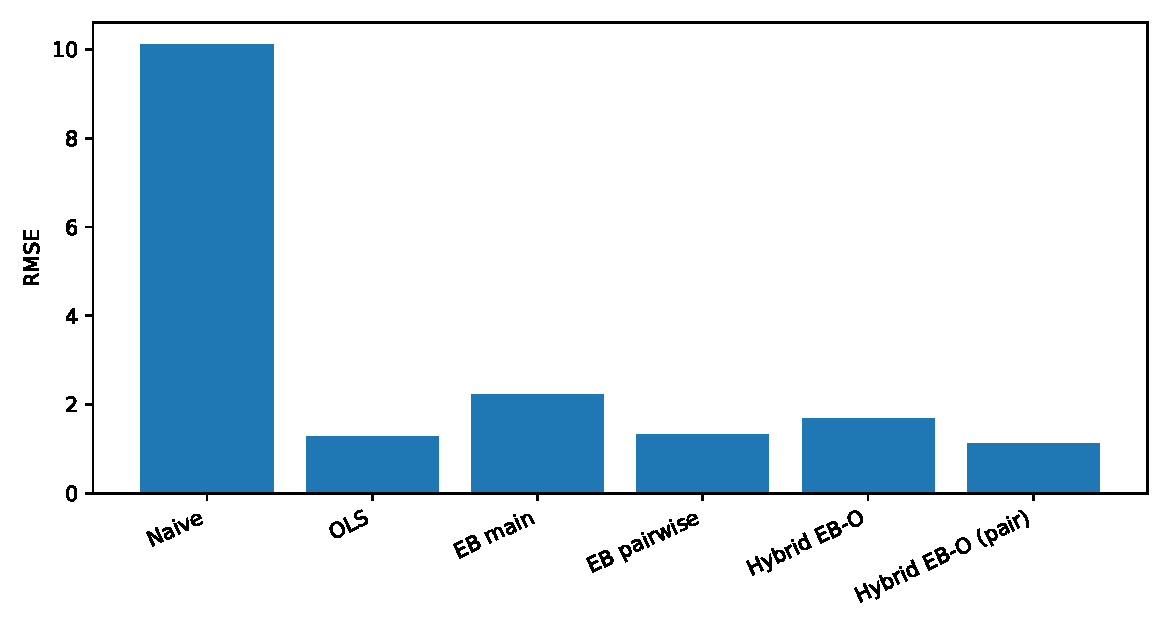
\includegraphics[width=\textwidth]{../OutputData/ks_fig_rmse_R1000.pdf}
\caption{RMSE.}
\end{subfigure}
\begin{subfigure}{0.48\textwidth}
\centering
\safeincludegraphics[width=\textwidth]{../OutputData/ks_fig_z_l2_R1000.pdf}
\caption{Mean latent $Z$ $L_2$ balance.}
\end{subfigure}
\caption{Kang--Schafer-style simulation results. The pairwise EB-offset hybrid starts from fixed pairwise EB and then applies adaptive tree corrections with hard pairwise reprojection. Latent $Z$[...]
\label{fig:ks-r1000}
\end{figure}

\subsection{Discussion}

The main lesson from the Kang--Schafer-style simulation is that the boosted tree layer can be combined with a strong fixed pairwise EB offset. With $B_{\max}=100$ and a smaller learning rate, the main[...] 

The result should be interpreted carefully. The hybrid methods do not use the outcome to choose tree splits, and they do not observe the true latent $Z$ variables. Therefore, the lower RMSE of th[...]

The simulation also highlights a useful tradeoff. The pairwise EB-offset hybrid has effective sample size similar to pairwise EB and improves RMSE in this design, while preserving exact pairwise [...]


\section{Real-data-based evaluation using ACS microdata}

The preceding simulation is useful because it controls the data-generating mechanism. However, a method intended for calibration and distribution alignment should also be examined under realistic cova[...] 

This analysis should be interpreted as a \emph{real-data-based semi-synthetic} study rather than as a causal analysis. The covariates and outcome are real ACS records, but the source sample is generat[...] 

The target estimand is the full-sample mean income. We also report the mean of $\log(1+\mathrm{income})$ as a sensitivity measure because income is highly right-skewed. The source sample size is $n=45[...]$

We compare five estimators. The first is the unweighted biased-source mean. The second is main-effect EB, which balances the observed main-effect covariate functions. The third is fixed pairwise [...]

\begin{table}[H]
\centering
\caption{Real-data-based ACS microdata analysis using $R=1000$ biased source samples of size $n=450$. The full adult ACS sample is treated as the pseudo-population benchmark. Income RMSE is in do[...]
\label{tab:acs-realdata}
\resizebox{\textwidth}{!}{%
\begin{tabular}{lrrrrrrrr}
\toprule
Method & Income bias & Income RMSE & Log-income RMSE & Main $L_2$ & Pair $L_2$ & Validation TV & Mean ESS & Mean max weight \\
\midrule
Biased source & 15045.3 & 15127.3 & 1.421 & 0.9365 & 1.0600 & 0.1124 & 450.0 & 0.0022 \\
Main-effect EB & -1980.9 & 2199.6 & 0.091 & $5.16\times10^{-9}$ & 0.5426 & 0.0149 & 268.0 & 0.0131 \\
Fixed pairwise EB & -128.4 & 1092.2 & 0.120 & $5.89\times10^{-5}$ & $7.39\times10^{-5}$ & 0.0073 & 197.9 & 0.0226 \\
EB-offset hybrid: main & -946.6 & 1406.6 & 0.100 & $7.09\times10^{-9}$ & 0.3633 & 0.0100 & 246.0 & 0.0150 \\
EB-offset hybrid: pairwise & -37.5 & 1130.9 & 0.118 & $5.89\times10^{-5}$ & $7.39\times10^{-5}$ & 0.0065 & 192.5 & 0.0227 \\
\bottomrule
\end{tabular}%
}
\end{table}

\begin{figure}[H]
\centering
\begin{subfigure}{0.48\textwidth}
\centering
\safeincludegraphics[width=\textwidth]{../OutputData/acs_fig_rmse_income.pdf}
\caption{RMSE for mean income.}
\end{subfigure}
\begin{subfigure}{0.48\textwidth}
\centering
\safeincludegraphics[width=\textwidth]{../OutputData/acs_fig_validation_tv.pdf}
\caption{Validation leaf imbalance.}
\end{subfigure}
\caption{Real-data-based ACS analysis. The pairwise EB-offset hybrid starts from fixed pairwise EB, preserves the pairwise constraints, and achieves the lowest validation leaf imbalance, while th[...]
\label{fig:acs-realdata-main}
\end{figure}

\begin{figure}[H]
\centering
\begin{subfigure}{0.48\textwidth}
\centering
\safeincludegraphics[width=\textwidth]{../OutputData/acs_fig_ess.pdf}
\caption{Mean effective sample size.}
\end{subfigure}
\begin{subfigure}{0.48\textwidth}
\centering
\safeincludegraphics[width=\textwidth]{../OutputData/acs_fig_error_boxplot.pdf}
\caption{Error distribution for mean log income.}
\end{subfigure}
\caption{Weight stability and error distribution in the ACS analysis. The pairwise EB-offset hybrid behaves like a tree-corrected version of fixed pairwise EB with hard pairwise reprojection, whereas [...]
\label{fig:acs-realdata-stability}
\end{figure}

The main finding is that all weighting methods dramatically reduce the bias of the raw source sample. The biased source mean overestimates mean income by about \$15,045 and has RMSE about \$15,12[...]

Fixed pairwise EB performs best for mean income in this particular ACS experiment, with income RMSE about \$1,092 and validation total variation 0.0073. The pairwise EB-offset hybrid has income R[...]

This ACS analysis clarifies the practical role of the proposed method. In applications where analysts already know the critical interactions, fixed-moment EB may be preferable. In applications wh[...]

\section{Interpretation of the simulation and ACS studies}

The Kang--Schafer-style simulation and the ACS real-data-based analysis support several conclusions.

First, the Kang--Schafer-style simulation shows that adaptive tree balance functions can be useful when relevant structure is hidden by nonlinear transformations of latent covariates. The pairwis[...]

Second, the ACS microdata analysis shows how the method behaves under real covariate distributions. With 1000 biased source samples, the main EB-offset hybrid improves substantially over main-eff[...]

Third, the hybrid hard-projection step is important. Flexible tree corrections can disturb the trusted calibration moments, whereas the hybrid versions restore the selected main-effect or pairwis[...]

Fourth, the method should not be viewed as universally superior to fixed-moment EB. If the analyst already knows a sufficiently informative balance basis, fixed-moment calibration may perform as [...]

Finally, there is a clear balance-stability tradeoff. Richer balance can require more variable weights and a lower ESS. The goal is therefore not to maximize ESS alone, but to find a useful trade[...] 

\section{Limitations}

The proposed method has several limitations.

\textbf{Target moments for tree leaves are required.} The method can only balance a tree-defined cell if a target moment for that cell is available or can be derived from an accepted target-momen[...]

\textbf{The algorithm is greedy.} The tree sequence is path-dependent. Different split criteria, learning rates, depths, or random seeds may produce different selected regions. Stability diagnost[...]

\textbf{Hard projection requires feasibility.} The projection step assumes that the hard main-effect constraints are feasible under the current support. If the hard target moments lie outside the conv[...] 

\textbf{Tree leaves can be sparse.} Small leaves can produce large multiplicative updates. Minimum leaf-mass rules, shrinkage, maximum-weight diagnostics, and ESS stopping rules are necessary.

\textbf{The method does not automatically balance all interactions.} It balances interactions that are found by the tree sequence and for which target moments are available. Important regions can stil[...] 

\textbf{Inference after adaptive selection is nontrivial.} Because the balance functions are selected adaptively, standard uncertainty formulas for fixed calibration may not directly apply. Bootstrap [...]

\section{Extensions}

Several extensions are natural.

\subsection{Selected-leaf final refit}

One alternative to projecting after every tree update is to use boosting only for feature discovery. After the boosting path is complete, collect the selected leaf indicators and run one final entropy[...] 

\subsection{Weight bounds}

The hybrid method can be combined with bounded weights. For example, the hard projection could impose
\begin{equation*}
